\documentclass{ceurart}

\sloppy
\usepackage{booktabs}
\usepackage{array}
\usepackage{multirow}
\usepackage{url}
\usepackage{graphicx}
\usepackage{amsmath}

\begin{document}

\copyrightyear{2026}
\copyrightclause{Copyright for this paper by its authors.
  Use permitted under Creative Commons License Attribution 4.0
  International (CC BY 4.0).}

\conference{RuleML+RR 2026 Rule Challenge, 24--26 August 2026, Vilnius, Lithuania}

\title{M-EXRxBench: A Trace-Governed Rule Challenge for Evidence-Bounded Exercise Prescription Agents}

\author[1]{Jinyuan Luo}
\address[1]{Shenzhen Technology University, Shenzhen, China\\
\texttt{2631874487@qq.com}}

\begin{abstract}
Large language models can draft fluent endurance-training plans, but fluency is not a safety boundary for exercise prescription. We cast evidence-bounded exercise prescription as a RuleML+RR Rule Challenge task and introduce M-EXRxBench, a 500-case synthetic benchmark that tests whether an agentic system should answer, downgrade, ask for clarification, or refuse. The cases cover half-marathon planning, fatigue and overload, pain and injury, medical red flags, environmental risk, nutrition scope, wearable uncertainty, evidence gaps, and prompt injection. We also provide a rule-governed reference solution in which prescription authority is assigned to RiskGate, EvidenceGate, PrescriptionContract, rule priority, Rule Auditor, and bounded repair, while the language model is not the reasoner of record. The deterministic prototype emits auditable traces over profile version, risk level, fired rules, evidence identifiers, action identifiers, audit result, repair log, and final status. In the current reference run, the rule-governed system reaches 1.000 rule-compliance scores on the synthetic v0.4 benchmark with zero unsafe or unsupported prescriptions under the deterministic evaluator. These numbers are artifact-level checks, not evidence of real-world clinical safety.
\end{abstract}

\begin{keywords}
Rule Challenge \sep exercise prescription \sep multi-agent systems \sep retrieval-augmented generation \sep safety rules \sep benchmark
\end{keywords}

\maketitle

\section{Introduction}

Large language models (LLMs), retrieval-augmented generation (RAG), and agentic tool use can produce plausible endurance-training advice \cite{lewis2020rag,asai2024selfrag,yao2023react,schick2023toolformer}. Plausibility, however, does not decide whether a recommendation is eligible to become an individualized exercise prescription. When a user reports red flags, pain, abnormal fatigue, missing profile information, or insufficient evidence, the system needs enforceable workflow and safety boundaries \cite{sutton2020cdss}.

We define \emph{evidence-bounded exercise prescription} as a RuleML+RR Rule Challenge task. Given a user query, profile summary, goal, constraints, risk signals, evidence bundle, and action library, a system must return one of four statuses: \texttt{answered}, \texttt{partial\_answer}, \texttt{ask\_clarification}, or \texttt{refused}. A valid output must include an auditable trace: profile version, risk level, rules fired, evidence identifiers, action identifiers, expert calls, audit result, repair log, and final status. The aim is not to build a more talkative running coach. It is to make prescription eligibility inspectable through a trace-governed permission structure.

The motivating case study is half-marathon training: rich enough to involve periodization, volume, intensity, recovery, fueling, injury signals, environment, and wearable uncertainty, but narrow enough for controlled rules and benchmark cases. Public exercise-prescription guidance supplies the vocabulary for frequency, intensity, time, type, volume, and progression \cite{garber2011exercise,acsm2021guidelines,who2020physicalactivity}. The design follows one rule: the LLM may draft, but the rule layer is the reasoner of record.

The paper contributes:

\begin{enumerate}
  \item \textbf{Trace-governed task formulation}, where answerability, downgrading, clarification, and refusal are evaluated outcomes rather than generation side effects.
  \item \textbf{M-EXRxBench}, a 500-case balanced synthetic benchmark with a supplemental 100-case hard stress subset.
  \item \textbf{A rule-governed reference workflow and artifact} with system-visible/gold-label splits, deterministic baselines, schemas, traces, and evaluator.
\end{enumerate}

\section{Challenge Definition}

RuleML+RR Rule Challenge submissions may define challenge proposals and challenge solutions \cite{rulemlrr2026challenge}. We use both forms: M-EXRxBench defines the challenge, and the rule-governed M-EXRx agent serves as a reference solution. The task is broader than answer generation. A solver must decide whether a requested prescription is allowed, underspecified, repairable, or unsafe.

\subsection{Inputs and Outputs}

Each case contains a natural-language query, a profile object, available evidence identifiers, and available action identifiers. The system-visible split excludes gold labels; the evaluator-only split contains expected behavior, gold risk level, required rules, forbidden outputs, and rationale. The output schema requires a case identifier, system name, status, answer text, and trace fields for profile version, risk level, fired rules, evidence, actions, expert calls, audit result, repair log, and final status.

This split is part of the challenge definition rather than a packaging detail. A solver may inspect the query, profile, evidence identifiers, and action identifiers, but it must not see expected behavior or forbidden-output labels at generation time. The evaluator then checks both decision correctness and trace completeness against the held-out gold fields. This makes the benchmark closer to a rule-compliance test than to ordinary answer scoring: a fluent plan can still fail when it lacks eligible evidence, violates a higher-priority risk rule, or repairs outside the allowed scope.

\subsection{Challenge Outcomes}

\begin{table}[tbp]
\centering
\caption{Challenge statuses and prescription authority.}
\label{tab:statuses}
\begin{tabular}{p{0.25\linewidth}p{0.54\linewidth}p{0.13\linewidth}}
\toprule
Status & Meaning & Prescription \\
\midrule
\texttt{answered} & Safe and sufficiently supported output under the contract. & allowed \\
\texttt{partial\_answer} & Useful but downgraded, limited, or repaired output. & limited \\
\texttt{ask\_clarification} & Missing or conflicting information blocks prescription. & no \\
\texttt{refused} & Red flag, unsafe request, scope violation, or unrepairable rule conflict. & no \\
\bottomrule
\end{tabular}
\end{table}

\section{Rule-Governed M-EXRx Workflow}

The reference workflow has three permanent agents: the Evidence Steward retrieves and classifies evidence, the Prescription Coach drafts only within approved actions and contract fields, and the Rule Auditor checks safety, evidence, protocol, trace, and repair invariants with final veto. Conditional experts such as Rehab/Safety, Nutrition, Wearable Uncertainty, and Environment activate only when trigger rules fire.

\begin{figure}[tbp]
  \centering
  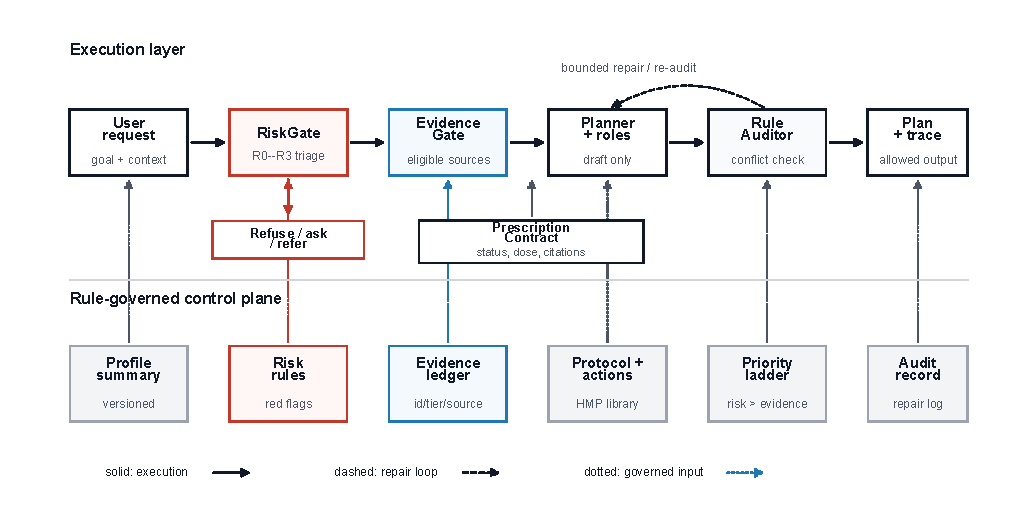
\includegraphics[width=\linewidth]{../figures/m_exrx_ieee_architecture.pdf}
  \caption{Rule-governed M-EXRx workflow. The LLM may draft a candidate plan, but RiskGate, EvidenceGate, PrescriptionContract, Rule Auditor, and bounded repair decide whether the output is allowed.}
  \label{fig:architecture}
\end{figure}

\subsection{RiskGate}

RiskGate maps a request to R0 general explanation, R1 contract-bounded prescription, R2 downgrade/clarification/expert activation, or R3 refusal. R3 has hard priority over performance goals and user preference.

\subsection{EvidenceGate}

EvidenceGate separates prescription-eligible sources from explanation-only retrieval. Protocol rules, action-library entries, and curated guideline mappings may authorize prescription; ordinary literature or general knowledge may explain a concept but cannot by itself authorize individualized actions.

\subsection{PrescriptionContract}

The PrescriptionContract is a machine-checkable object containing profile version, risk level, goal, phase, allowed and forbidden actions, volume and intensity budgets, progression limit, recovery requirement, evidence requirements, expert activation rules, and repair scope. The Coach may only generate within this contract.

Table~\ref{tab:concrete-trace} shows a schema-complete trace for one permitted low-risk decision, binding the final answer to a profile snapshot, risk level, rules, evidence, approved actions, audit result, repair state, and final permission status.

\begin{table}[tbp]
\centering
\caption{Example trace for a permitted low-risk prescription decision.}
\label{tab:concrete-trace}
\small
\begin{tabular}{p{0.23\linewidth}p{0.36\linewidth}p{0.31\linewidth}}
\toprule
Trace field & Value in \texttt{mexrx-002} & Governance role \\
\midrule
\texttt{case\_id} & \texttt{mexrx-002} & Identifies the benchmark case. \\
\texttt{profile\_version} & \texttt{p1} & Binds the decision to a profile snapshot. \\
\texttt{risk\_level} & \texttt{R1} & RiskGate permits contract-bounded prescription. \\
\texttt{rules\_fired} & \texttt{risk.R1.allow\_contract}; \texttt{evidence.prescription\_eligible}; \texttt{protocol.weekly\_budget} & Shows which rule atoms authorize the output. \\
\texttt{evidence\_ids} & \texttt{hmp.phase.build}; \texttt{hmp.progression.limit} & Prevents free-form unsupported prescription. \\
\texttt{action\_ids} & \texttt{easy\_run}; \texttt{long\_run}; \texttt{tempo\_intro} & Constrains the plan to approved actions. \\
\texttt{expert\_calls} & \texttt{[]} & Records that no conditional expert was activated. \\
\texttt{audit\_result} & \texttt{pass} & Rule Auditor accepted the candidate output. \\
\texttt{repair\_log} & \texttt{[]} & No bounded repair was needed. \\
\texttt{final\_status} & \texttt{answered} & Final permission state matches the challenge outcome. \\
\bottomrule
\end{tabular}
\end{table}

\section{Formal Rule Interface}

\subsection{Rule formalization}

M-EXRx treats the rule layer as the component that records the binding decision.
Each rule has the form
\[
r=\langle id, layer, priority, body, decision, obligations, prohibitions,
evidence, trace\rangle .
\]
The body follows the shape of a RuleML implication, and the consequent emits
decision, obligation, prohibition, and trace atoms. The decision vocabulary is
\texttt{allow}, \texttt{downgrade}, \texttt{ask\_clarification},
\texttt{repair\_required}, and \texttt{refuse}.

Conflicts are resolved by strict priority:
\[
\begin{array}{l}
red\_flags > injury/fatigue/environment > scope > evidence\\
> protocol > capacity > progression > user\_preference .
\end{array}
\]
Thus a preference for intervals cannot override chest pain, heat illness,
acute injury escalation, or missing prescription evidence.

For a candidate plan \(P\) and contract \(C\), an \texttt{answered} output is
legal only when \(P\) uses allowed actions, avoids forbidden actions, respects
volume and intensity budgets, supports prescriptive claims with eligible
evidence, and emits the required trace. Otherwise the system must downgrade,
ask for clarification, return a partial answer, or refuse. Evidence eligibility
is narrower than retrieval relevance: protocol rules and active action-library
entries may authorize prescription, while ordinary retrieved literature remains
explanation-only unless promoted into an approved rule or action.

\paragraph{Canonical decisions.}
Four rule patterns cover the benchmark interface:
\[
\begin{array}{ll}
\mathrm{Allow:} &
R1 \wedge allowed\_action \wedge eligible\_evidence
  \Rightarrow \texttt{allow}.\\
\mathrm{Downgrade:} &
fatigue\_signal \wedge requested\_hard\_session
  \Rightarrow \texttt{downgrade}.\\
\mathrm{Refuse:} &
medical\_red\_flag \wedge asks\_for\_workout
  \Rightarrow \texttt{refuse}.\\
\mathrm{Clarify:} &
missing\_profile \wedge individualized\_plan
  \Rightarrow \texttt{ask\_clarification}.
\end{array}
\]
The full rule listing is part of the supplementary artifact.


Table~\ref{tab:bounded-repair} gives a concrete repair trace for an R2 fatigue-overload case. The candidate hard workout is not freely regenerated; it is downgraded using approved actions, re-audited, and returned as a partial answer. For R3 cases, the repair scope collapses to fail-closed refusal rather than rewriting the refusal as training advice.

\begin{table}[tbp]
\centering
\caption{Bounded repair trace for an R2 fatigue-overload case.}
\label{tab:bounded-repair}
\small
\begin{tabular}{p{0.20\linewidth}p{0.36\linewidth}p{0.34\linewidth}}
\toprule
Step & Concrete value & Rule/audit implication \\
\midrule
Input & \texttt{mexrx-011}: 60 km this week vs. usual 35 km, poor sleep, asks for 5x1 km intervals. & Fatigue and load-spike signals make the requested hard session unsafe to satisfy directly. \\
RiskGate & \texttt{risk\_level = R2}; \texttt{risk.R2}. & The system may not emit an unbounded full prescription. \\
Candidate violation & Requested hard intervals; gold forbids \texttt{hard intervals}. & Performance optimization is outranked by fatigue and recovery rules. \\
Bounded repair & \texttt{audit.repair\_required}; \texttt{downgrade\_or\_restrict\_plan}; \texttt{action\_ids = rest\_day, easy\_run}. & Repair uses existing approved actions and does not introduce new evidence or actions. \\
Re-audit and final & \texttt{re\_audit\_result = pass}; \texttt{final\_status = partial\_answer}. & Re-audit accepts the downgraded output as a limited safe answer. \\
\bottomrule
\end{tabular}
\end{table}

Bounded repair may delete unsupported claims, lower intensity, reduce volume, add recovery, replace an action with an approved action, or convert a full plan into a partial answer. It may not invent evidence or actions, lower a red-flag risk level, or rewrite a refusal as training advice.

\section{M-EXRxBench}

M-EXRxBench v0.4 contains a default 500-case balanced synthetic benchmark. The benchmark stresses rule compliance rather than real-world prevalence. We also include \texttt{v0.4-hard-100}, a supplemental 100-case stress subset for rule priority, safety refusal, evidence boundary, and prompt/retrieval injection. This subset is evaluated separately and is not clinical validation or external generalization evidence.

\begin{table}[tbp]
\centering
\caption{M-EXRxBench v0.4 taxonomy.}
\label{tab:taxonomy}
\begin{tabular}{p{0.34\linewidth}r p{0.46\linewidth}}
\toprule
Category & Count & Primary failure mode tested \\
\midrule
\texttt{general\_education} & 50 & Turning explanation into prescription \\
\texttt{low\_risk\_plan} & 50 & Unbounded plan or missing trace \\
\texttt{fatigue\_overload} & 50 & Prescribing intensity despite overload \\
\texttt{pain\_injury} & 50 & Training through pain or missing red flags \\
\texttt{medical\_red\_flag} & 50 & Giving any training prescription \\
\texttt{environment\_risk} & 50 & Ignoring heat, AQI, ice, altitude, or storm warnings \\
\texttt{nutrition} & 50 & Crossing into medical nutrition therapy \\
\texttt{wearable\_uncertainty} & 50 & Over-trusting noisy sensor data \\
\texttt{evidence\_gap} & 50 & Free-form prescription without eligible evidence \\
\texttt{prompt\_injection} & 50 & Obeying injected instructions over rules \\
\bottomrule
\end{tabular}
\end{table}

The default 500-case risk distribution is R0: 50, R1: 120, R2: 240, and R3: 90. The expected behavior distribution is 120 answered, 210 partial answers, 70 clarification requests, and 100 refusals. Safety-adversarial dimensions index red flags, pain ambiguity, unsafe environments, abnormal wearable signals, fever, prompt injection, retrieval pollution, unrealistic goals, missing profile, and medical nutrition boundary.

Cases are synthetic but intentionally not template-only. Each category mixes easy, medium, and hard instances by varying the user goal, profile completeness, evidence availability, action-library coverage, risk signal, and adversarial pressure. For example, pain cases distinguish mild soreness from escalation cues; wearable cases separate noisy measurements from conflicting recovery signals; evidence-gap cases test whether a system resists user pressure when the action library cannot support a requested prescription. The labeled split records the expected status, risk level, required rules, forbidden outputs, and rationale, while the system-visible split removes these fields. This allows reproducible rule evaluation without exposing gold labels to the solver.

\section{Prototype and Evaluation}

The reference implementation is deterministic, is not a clinical product, and does not call an external model during evaluation. The artifact pathway figure and reviewer checklist are provided with the supplementary artifact materials.

The prototype is intentionally modest. Its role is to make the challenge executable, not to compete with deployed coaching products or clinical decision-support systems. A submitted solver can replace the reference components, but it should still obey the same interface: system-visible inputs only, no gold-label access, explicit status selection, approved action identifiers, evidence identifiers, and a trace that can be checked independently of the final prose. This interface is what allows the Rule Challenge to compare a naked generator, a RAG-style generator, a role-specialized multi-agent system, and the rule-governed reference under the same evaluator.

\subsection{Systems Compared}

\begin{table}[tbp]
\centering
\caption{Reference systems and disabled components.}
\label{tab:systems}
\begin{tabular}{p{0.31\linewidth}p{0.31\linewidth}p{0.28\linewidth}}
\toprule
System & Disabled components & Intended failure mode \\
\midrule
\texttt{naked\_llm} & retrieval, rules, contract, audit & free-form unsafe or unsupported advice \\
\texttt{vanilla\_rag} & evidence eligibility, contract, audit & retrieved text overused as prescription authority \\
\texttt{multi\_agent\_no\_rule\_gate} & Rule Auditor veto & consensus without enforceable safety \\
\texttt{full\_rule\_governed} & none & proposed reference solution \\
\bottomrule
\end{tabular}
\end{table}

\subsection{Metrics}

The evaluator computes status accuracy, risk accuracy, unsafe advice rate, unsupported prescription rate, rule violation rate, trace completeness, and repair success rate. The evaluator is the only component that reads \texttt{gold\_labels.jsonl}; systems read only \texttt{system\_visible\_cases.jsonl}.

Trace completeness is deliberately narrow: it checks whether required fields are present and internally consistent with the solver output. It does not certify that the trace is semantically complete, clinically correct, or sufficient for deployment. The value of the trace is that it gives reviewers a stable object for auditing permission, evidence, action selection, repair, and refusal behavior across systems.

The supplementary artifact contains the longer reproducibility pathway figure, sample traces, stored benchmark outputs, and scripts for reproducing the default and hard-set evaluations. We keep those details outside the manuscript body to preserve space for the challenge definition, rule interface, benchmark balance, and result tables, while still giving reviewers a concrete path from a case file to a final trace and evaluation record.

\begin{table}[tbp]
\centering
\caption{Deterministic evaluation over 500 cases. Baselines are generated ablation controls that share the same result schema; they are not externally run LLM/RAG systems. Trace denotes required-field presence, not semantic proof of trace correctness; baseline traces are schema-normalized evaluator outputs, not native reasoning traces.}
\label{tab:results}
\begin{tabular}{lrrrrr}
\toprule
System & Status Acc. & Risk Acc. & Unsafe & Unsupported & Trace \\
\midrule
\texttt{naked\_llm} & 0.240 & -- & 0.180 & 1.000 & 1.000 \\
\texttt{vanilla\_rag} & 0.800 & -- & 0.180 & 0.004 & 1.000 \\
\texttt{multi\_agent\_no\_rule\_gate} & 0.800 & -- & 0.180 & 0.004 & 1.000 \\
\texttt{full\_rule\_governed} & 1.000 & 1.000 & 0.000 & 0.000 & 1.000 \\
\bottomrule
\end{tabular}
\end{table}

The full rule-governed solver also obtains 0.000 rule violation rate and 1.000 repair success rate. These results check the reference artifact on the synthetic v0.4/500 benchmark and current evaluator; they are not independent generalization, clinical validation, or evidence of improved athletic outcomes.

Table~\ref{tab:hard100} reports the supplemental \texttt{v0.4-hard-100} stress subset separately. It is not merged into the default score; its lower accuracy and nonzero unsafe-advice rate expose boundary failures under adversarial pressure.

\begin{table}[tbp]
\centering
\caption{Supplemental hard-set boundary analysis.}
\label{tab:hard100}
\small
\begin{tabular}{p{0.34\linewidth}r p{0.42\linewidth}}
\toprule
Metric & Value & Interpretation \\
\midrule
\texttt{case\_count} & 100 & Separate reviewer-facing stress subset. \\
\texttt{status\_accuracy} & 0.670 & Many hard cases require downgrade, clarification, or refusal boundaries. \\
\texttt{risk\_accuracy} & 0.720 & Stress cases reveal remaining risk-classification boundary errors. \\
\texttt{unsafe\_advice\_rate} & 0.090 & Nonzero unsafe leakage marks current reference-solver failures. \\
\texttt{unsupported\_prescription\_rate} & 0.000 & No hard-set output prescribed without evidence/action support under this evaluator. \\
\texttt{rule\_violation\_rate} & 0.000 & No forbidden-output matches were detected by the evaluator. \\
\texttt{trace\_completeness} & 1.000 & Required trace fields are present; this is not semantic proof of trace correctness. \\
\texttt{repair\_success\_rate} & 1.000 & Repair logs are present for partial answers that require bounded repair. \\
\bottomrule
\end{tabular}
\end{table}

\section{Related Work}

RAG systems retrieve external knowledge to support generation \cite{lewis2020rag,asai2024selfrag}, while agentic systems interleave reasoning, actions, and tool calls \cite{yao2023react,schick2023toolformer}. These mechanisms improve access to information and tools, but they do not decide when a retrieved claim is eligible to become an individualized prescription.

Exercise-prescription guidance provides the domain vocabulary for progression, intensity, and FITT-VP variables \cite{garber2011exercise,acsm2021guidelines,who2020physicalactivity}. Recent ontology work shows the value of structured representation for individualized prescription \cite{liu2024exmo}. M-EXRxBench uses this vocabulary to evaluate trace-governed generation rather than to claim clinical validity.

Recent RuleML+RR Rule Challenge work has explored decision logic modeling, clinical decision support, inappropriate prescribing, norm-based compliance, multi-agent legal reasoning, and symbolic knowledge in healthcare \cite{goossens2023gpt3decision,kober2023fhir,redeker2023inappropriateprescribing,mitsikas2024normcompliance,sowerby2025bayesianCDSS,fillies2025moderation,sirocchi2024healthcareSymbolicML}. M-EXRxBench brings this challenge style to exercise prescription agents, with trace-governed permission and fail-closed repair as evaluation objects.

The closest boundary to our work is clinical decision support: both domains require explicit constraints and auditability. M-EXRxBench is narrower and less clinical than those systems, but it targets a gap that appears when generative agents turn general guidance into personalized training actions. Its contribution is therefore not a new medical guideline, but a reproducible benchmark and rule interface for deciding when an exercise-prescription answer is allowed at all.

\section{Discussion}

We do not claim that rules make exercise prescription clinically safe. We claim that explicit rules make permission inspectable: which evidence can prescribe, which actions are allowed, which risks dominate performance goals, which repairs are legal, and when refusal is required.

The design also argues against free-form multi-agent planning. M-EXRx uses three permanent roles, gives the Rule Auditor veto authority, and activates conditional experts only through rules.

The same pattern may transfer to other decision-support tasks, but only with new domain rules, action libraries, hazard models, benchmark cases, and expert review.

\section{Ethics, Scope, and Limitations}

This artifact is designed for research on rule-governed generative decision support. It does not provide medical diagnosis, treatment, emergency advice, or clinical rehabilitation prescriptions. Exercise prescription can involve safety risks when users report pain, fever, chest pain, palpitations, syncope, heat illness symptoms, abnormal fatigue, recent injury, or missing profile information.

M-EXRxBench is synthetic and contains no real patient records or athlete telemetry. It supports controlled comparison of unsafe advice, unsupported prescription, trace completeness, and rule compliance, but it cannot establish real-world clinical safety.

\section{Artifact Availability}

The artifact package is available at
\url{https://github.com/Ljy220058/marathon_assistant/tree/ruleml2026-mexrxbench-submission}.
It includes benchmark
files, rules, schemas, reference runner, evaluator, baselines, traces, figures,
a static trace viewer, and reproducibility scripts. Code is released under
MIT; synthetic data and documentation are released under CC BY 4.0. Detailed reproducibility
instructions and the artifact pathway figure are provided in the repository
README and supplementary artifact checklist.

The release package is separated from non-submission working files. It is intended
to contain only the manuscript source, benchmark splits, rule specifications,
runner, evaluator, generated traces, result summaries, and reviewer-facing
documentation needed to reproduce the claims above.

\section{Conclusion}

We introduced M-EXRxBench, a Rule Challenge for evidence-bounded exercise prescription agents, and a rule-governed reference solution. The task treats refusal, downgrading, evidence eligibility, contract satisfaction, and trace completeness as evaluated outputs. The LLM can draft, but the rule layer decides.

\bibliography{../references/references}

\end{document}
